% \begin{figure}[!tbp]
% \centering
%     \begin{minipage}[t]{0.242\textwidth}
%     \centering
%     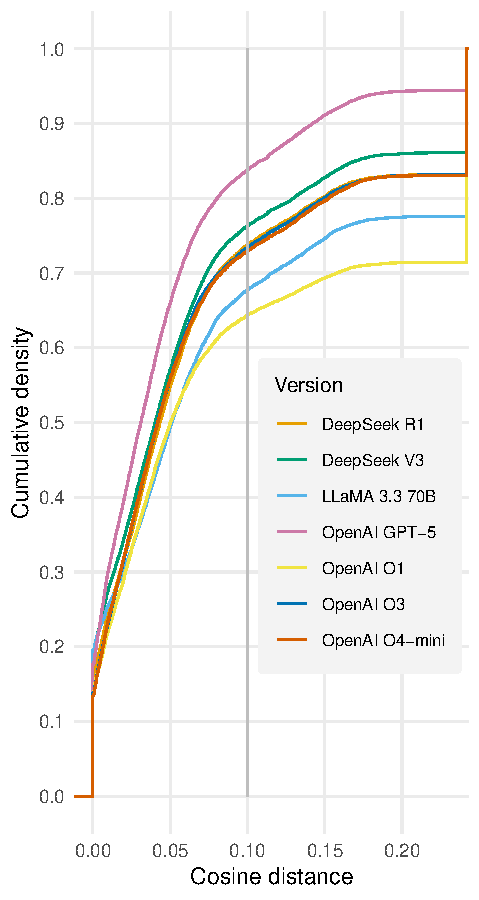
\includegraphics[page=1, width=\linewidth]{Plots_tables/pmoa_updated_man_figs.pdf}
%     \end{minipage}
%     \hfill
%     \begin{minipage}[t]{0.242\textwidth}
%     \centering
%     \includegraphics[page=2, width=\linewidth]{Plots_tables/pmoa_updated_man_figs.pdf}
%     \end{minipage}
%     \hfill
%     \begin{minipage}[t]{0.242\textwidth}
%     \centering
%     \includegraphics[page=3, width=\linewidth]{Plots_tables/pmoa_updated_man_figs.pdf}
%     \end{minipage}
%     \hfill
%     \begin{minipage}[t]{0.242\textwidth}
%     \centering
%     \includegraphics[page=4, width=\linewidth]{Plots_tables/pmoa_updated_man_figs.pdf}
%     \end{minipage}
%     \caption{Comparison of different LLM for extracting temporal clinical events from case reports. From left to right: (\textbf{A}) event match cumulative distribution function, (\textbf{B}) concordance box plots, (\textbf{C}) time discrepancy from manual annotation timestamps among matched events (overall), and (\textbf{D}) time discrepancy disaggregated by clinician annotator timestamp (time from presentation). 
%     %\textcolor{red}{Have same figure for LAPJV?}
%     }
%     \label{fig:tts_evaluation}
%     \vspace{-10pt}
% \end{figure}



\begin{figure}[!tbp]
\centering

% First row: panels A and B
\begin{minipage}[t]{0.49\linewidth}
    \centering
    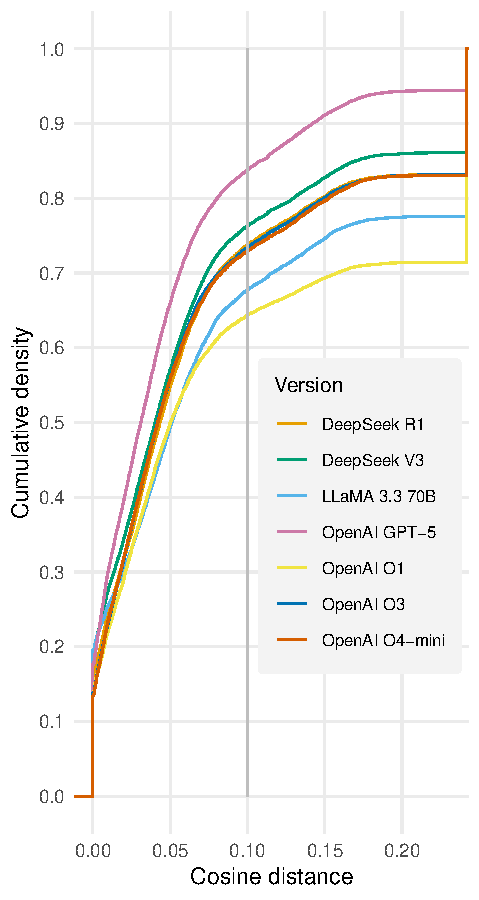
\includegraphics[
        page=1,
        width=0.8\linewidth
    ]{Plots_tables/pmoa_updated_man_figs.pdf}
\end{minipage}
\hfill
\begin{minipage}[t]{0.49\linewidth}
    \centering
    \includegraphics[
        page=2,
        width=0.8\linewidth
    ]{Plots_tables/pmoa_updated_man_figs.pdf}
\end{minipage}

\par\medskip

% Second row: panels C and D
\begin{minipage}[t]{0.49\linewidth}
    \centering
    \includegraphics[
        page=3,
        width=0.8\linewidth
    ]{Plots_tables/pmoa_updated_man_figs.pdf}
\end{minipage}
\hfill
\begin{minipage}[t]{0.49\linewidth}
    \centering
    \includegraphics[
        page=4,
        width=0.8\linewidth
    ]{Plots_tables/pmoa_updated_man_figs.pdf}
\end{minipage}

\caption{
Comparison of different LLMs for extracting temporal clinical events
from case reports:
(\textbf{A}) cumulative distribution of event-matching cosine distances;
(\textbf{B}) temporal-concordance box plots;
(\textbf{C}) timestamp discrepancies between model-generated and manual
annotations among semantically matched events; and
(\textbf{D}) timestamp discrepancies stratified by the clinician-annotated
time relative to presentation.
}
\label{fig:tts_evaluation}
\vspace{-10pt}
\end{figure}